\documentclass[13pt]{extreport}
\usepackage[utf8]{inputenc}
\usepackage[vietnamese,english]{babel}
%\usepackage{type1cm}
\usepackage[left=3.50cm, right=2.00cm, top=3.50cm, bottom=3.00cm]
{geometry}
%\usepackage[left=3.0cm, right=1.50cm, top=3.00cm, bottom=2.50cm]{geometry}
\usepackage{graphicx}
\usepackage{float}
\usepackage{mathrsfs} 
\usepackage{hyperref}
\usepackage{amsfonts}
\usepackage{longtable}
\usepackage[intlimits]{amsmath}
\usepackage{amsmath}
\DeclareMathOperator*{\argmax}{argmax} % thin space, limits underneath in displays
\usepackage{array}
\usepackage{amsxtra,amssymb,latexsym,amscd,amsthm}
\newtheorem{theorem}{\MakeUppercase{K}ết quả}[section]
\renewcommand{\baselinestretch}{1.5}
\usepackage{hyperref}

%——————–
\begin{document}
%tao khung
\newcommand{\Khung}[2]{
\begin{tabular}{|l|}
\hline\rule[-2ex]{0pt}{5.5ex}
\parbox{#1}{#2}\\
\hline
\end{tabular}
}

\Khung{.92\textwidth}{

\begin{center}
\normalsize
\textbf{TRƯỜNG ĐẠI HỌC BÁCH KHOA HÀ NỘI}\\
\normalsize
\textbf{VIỆN TOÁN ỨNG DỤNG VÀ TIN HỌC}\\
\textbf{------------------------------------------------------}\\[0.4cm]

\includegraphics[scale=.8]{logobkdentrang}\\[1.2cm]
\textbf{{\large ỨNG DỤNG MÔ HÌNH MARKOV ẨN\\TRONG VIỆC NHẬN DIỆN GIỌNG NÓI TIẾNG VIỆT
}}\\[0.3cm]
\textbf{}\\[1cm]
\textbf{{\large ĐỒ ÁN MÔN HỌC}}\\[0.2cm]
\textbf{{\large Chuyên ngành: TOÁN TIN}}\\[1cm]
\end{center}
\begin{flushleft}
\hspace{1.5 cm} \textbf{ Giáo viên hướng dẫn:\hspace{0.2cm}{ TS. NGUYỄN THỊ NGỌC ANH }}\\[0.2cm]
\hspace{1.5 cm} \textbf{ Sinh viên thực hiện:\hspace{0.5cm}{ NGUYỄN ANH TÚ\\\hspace{6 cm}PHẠM ANH TUẤN\\\hspace{6 cm}TRẦN TRỌNG CƯỜNG}}\\[0.2cm]
\hspace{1.5 cm} \textbf{ Lớp:\hspace{3.3cm}{ KSTN TOÁN TIN - K60}}\\
\end{flushleft}

\vspace{1.3cm}
\begin{center}
\textbf{{\large HÀ NỘI - 2018}}\\
\end{center}
 }
\thispagestyle{empty}
\newpage

\tableofcontents
\newpage

%\listoffigures

\newpage
\addcontentsline{toc}{chapter}{{\bf Mở đầu}}

\chapter*{Mở đầu}\
\par Lý thuyết của mô hình Markov ẩn đã được công bố do Baum vào khoảng đầu những năm 1970 và nó đã được vận dụng vào các bài toán xử lý giọng nói tự nhiên vào thời điểm đó. Tuy nhiên, mô hình Markov chỉ mới được thực sự công nhận vào những năm gần đây do sự cải tiến trong việc đưa những lý thuyết trên vào ứng dụng thực tế.
\par Trong bài báo cáo này, chúng tôi xin trình bày về mô hình Markov ẩn và ứng dụng của nó trong việc nhận diên giọng nói Tiếng Việt. Như chúng ta đã biết, giọng nói thường được miêu tả bằng một hàm biên độ phụ thuộc vào thời gian, và các phương pháp xử lý âm thanh sẽ đưa tín hiệu thành các vector liên tục. Chính vì lí do này, mô hình Markov ẩn rời rạc thông thường làm mất thông tin và nhận diện không chính xác. Điều đó đòi hỏi cần có một cách biểu diễn hàm mật độ các quan sát (tín hiệu âm thanh) của mô hình Markov ẩn. Bài báo này sẽ bàn luận về Gaussian Mixture Model - Hidden Markov Model, hay còn viết tắt là GMMHMM để giải quyết vấn đề này. Bên cạnh đó, chúng em cũng sẽ trình bày những cải tiến của mô hình giúp tăng khả năng nhận diện giọng nói Tiếng Việt.
\par Bố cục của bài báo cáo này gồm 5 chương. Chương 1 giới thiệu, định nghĩa và giải quyết ba bài toán quan trọng nhất trong mô hình Markov ẩn. Chương 2 nói về mô hình Gaussian hỗn hợp (GMM) và tích hợp nó vào mô hình Markov ẩn (GMMHMM). Chương 3 trình bày sơ qua về âm thanh và thuật toán MFCC để xử lý tiếng nói. Chương 4 đưa ra mô tả về model mà chúng tôi sử dụng để nhận diện từng từ đơn trong Tiếng Việt. Chương 5 miêu tả về bộ dữ liệu, ghi lại những kết quả thực nghiệm của mô hình, và cuối cùng chỉ ra những hướng nghiên cứu tiếp theo.
\par Mặc dù chúng em đã rất cố gắng hoàn thành đề tài nhưng do hạn chế về kinh nghiệm
và kiến thức nên bài không tránh khỏi nhiều thiếu sót cần được khắc
phục. Vì vậy chúng em mong thầy cô và các bạn đóng góp ý kiến để chúng em có thể làm tốt
hơn sau này.
\par Cuối cùng, chúng em xin trân trọng cám ơn sự hướng dẫn của TS. Nguyễn Thị Ngọc Anh để chúng em có thể hoàn thành bài báo cáo này.


\begin{flushright}
Hà Nội, ngày 8 tháng 6 năm 2018
\end{flushright}
%\addcontentsline{toc}{chapter}{{\bf Đặt vấn đề}}
%\chapter{Đặt vấn đề}
%\newpage
\chapter{Mô Hình Markov Ẩn}
Chương này sẽ giới thiệu các định nghĩa và giải quyết các bài toán cơ bản trong Mô hình Markov ẩn

\section{Mô Hình Markov Ẩn}
Một mô hình Markov ẩn gồm:
\begin{itemize}
\item N – số lượng trạng thái của mô hình. Ký hiệu các trạng thái là S =    \{  $ S_1$, $S_2$, …, $S_N $  \}   và trạng thái ở thời điểm t là $q_t$. \par
\item M – là số quan sát xảy ra ở mỗi trạng thái. Các quan sát này tương ứng là đầu ra của mô hình. Ký hiệu các tín hiệu quan sát này là V =    \{  $ v_1$, $v_2$, …, $v_M $  \}. \par
\item Ma trận xác suất chuyển trạng thái A =    \{  $  a_{ij}  $  \}    với : 
\begin{center}
${a_{ij}} = p{\rm{(}}{q_{t + 1}} = {S_j}{\rm{|}}{q_t} = {S_i}), \quad 1 \le i,j \le N$
\end{center}

\item Ma trận xác suất của các quan sát ở trạng thái $j$: B =  $  \{  $  $b_j(k)$  $  \}  $  với: 
  \begin{center}  
  
  \par${{\rm{b}}_{\rm{j}}}\left( {\rm{k}} \right) = {\rm{p(}}{{\rm{v}}_{\rm{k}}} \textrm{ ở thời điểm }{\rm{t}}{\rm{|}}{{\rm{q}}_{\rm{t}}} = {\rm{}}{{\rm{S}}_{\rm{j}}}), \quad{\rm{}}1 \le {\rm{j}} \le {\rm{N}},{\rm{}}1 \le {\rm{k}} \le {\rm{M}}$
  \end{center}
  \item Xác suất ban đầu của mỗi trạng thái: $\pi  = \left\{ {{\pi _i}} \right\}$
 với: \par
 \begin{center}
 

$  \pi _{i}=p \left( q_{1}=~S_{i} \right) ,\quad 1 \leq i \leq N $
 \par
  \end{center}
  \end{itemize}

  Với giá trị của N,M,A,B và $\pi$, mô hình Markov ẩn có thể sinh ra một chuỗi quan sát $${\rm{O}} = {\rm{O}}_{\rm{1}}{\rm{O}}_{\rm{2}}...{\rm{O}}_{\rm{T}} $$ (trong đó ${\rm{O}}_{\rm{t}}$ là một quan sát trong V, và T là số quan sát của chuỗi O) như sau:
  \begin{enumerate}
  \item Chọn trạng thái ban đầu ${\rm{q}}_{\rm{1}} = {\rm{S}}_{\rm{i}}$ theo xác suất ban đầu $\pi$.
  \item Đặt $t = 1$.
  \item Chọn $O_t=v_k$ theo xác suất ở trạng thái $S_j$ hay $b_i(k)$.
  \item Chuyển trạng thái mới $q_{t+1}=S_j$ theo xác suất chuyển trạng thái $a_{ij}$.
  \item Đặt $t=t+1$, nếu $t<T$ quay lại bước 3. 
  Ngược lại, dừng thủ tục.
  \end{enumerate}
  Để thuận tiện cho việc trình bày, ta quy ước mỗi mô hình HMM sẽ được đại diện bởi bộ tham số: $  \lambda = \left( A,B, \pi  \right)  $
. \par
  

\section{Ba bài toán cơ bản của HMM}


Để có thể áp dụng được mô hình HMM vào các ứng dụng phức tạp trong thực tế, trước hết cần có lời giải thỏa đáng cho 3 bài toán cơ bản của HMM: \par
\begin{itemize}
\item\textbf{Bài toán 1}: Cho trước chuỗi quan sát O =   $O_1$, $O_2$, …, $O_T$  và mô hình HMM $  \lambda = \left( A,B, \pi  \right)  $.
 Làm sao để tính toán hiệu quả $ p \left( O \vert  \lambda  \right)  $
 – xác suất xảy ra chuỗi O với mô hình $  \lambda  $ như trên
. \par
\item \textbf{Bài toán 2}: Cho trước chuỗi quan sát O =   $O_1$, $O_2$, …, $O_T$  và mô hình HMM $  \lambda = \left( A,B, \pi  \right) . $
 Cần tìm ra chuỗi trạng thái tối ưu Q = $q_1$, $q_2$, …, $q_T$   đã sinh ra O. \par
\item \textbf{Bài toán 3}: Cho trước chuỗi quan sát O =   $O_1$, $O_2$, …, $O_T$ . Làm thế nào để xác định mô hình $  \lambda = \left( A,B, \pi  \right)  $
 sao cho xác suất $ p \left( O \vert  \lambda  \right)  $ đạt giá trị lớn nhất.
\end{itemize}
\subsection{\textbf{{Bài toán 1}}} 
Mục tiêu của bài toán thứ nhất là tính $ p \left( O \vert  \lambda  \right)  $
 – xác suất phát sinh O từ mô hình $  \lambda  $
. Một cách đơn giản để giải quyết vấn đề này là trực tiếp duyệt qua tất cả các chuỗi trạng thái Q làm phát sinh ra O. Khi đó, xác suất $ p \left( O \vert  \lambda  \right)  $
 sẽ là tổng các xác suất phát sinh O từ tất cả các chuỗi Q khác nhau: 

 $$P\left( {O{\rm{|}}\lambda } \right) = \mathop \sum \limits_{\forall Q} P\left( {Q{\rm{|}}Q,\lambda } \right).P\left( {Q{\rm{|}}\lambda } \right)
     = \mathop \sum \limits_{{q_1},{q_2}, \ldots ,{q_t}} {\pi _{{q_1}}}{b_{{q_1}}}\left( {{O_1}} \right){a_{{q_1}{q_2}}}{b_{{q_2}}}\left( {{O_2}} \right) \ldots {a_{{q_T} - 1{q_T}}}{b_{{q_T}}}({O_T})$$
    
Để xác định $p(O|\lambda )$ theo cách trên, ta cần thực hiện $2T.N^T$ phép tính. Điều này là không khả thi ngay cả với các giá trị nhỏ của N (số trạng thái của mô hình) và T (chiều dài của chuỗi quan sát); chẳng hạn với N = 5 và T = 100, tổng số phép tính cần phải thực hiện là ${2.100.5^{100}}{\rm{}} \approx {\rm{}}{10^{72}}$
. Rõ ràng chi phí tính toán là quá lớn, ta không thể tính $ p \left( O \vert  \lambda  \right)  $
 theo cách như trên. \par
Một giải pháp khả thi hơn để tính $ p \left( O \vert  \lambda  \right)  $
 là thông qua thủ tục forward–backward.\\
\textbf{Thủ tục forward}: Ta định nghĩa biến forward $  \alpha_{t} \left( i \right)  $ như sau: $${\alpha _t}\left( i \right) = p{\rm{(}}{O_1}{O_2} \ldots {O_t},{q_t} = {S_i}{\rm{|}}\lambda ) $$
 là xác suất mà chuỗi O =   $O_1$, $O_2$, …, $O_t$ được quan sát ở trạng thái $S_i$ tại thời điểm $t$  từ mô hình $  \lambda  $ cho trước. 
Theo quy nạp, ta có thể tính được $\alpha_i(t)$ như sau: \par
\begin{enumerate}
\item Khởi tạo
$$ \alpha _{1} \left( i \right) =~ \pi _{i}b_{i} \left( O_{1} \right) ,~1 \leq i \leq N $$

\item Quy nạp:
\begin{equation}
\alpha _{t+1} \left( j \right) =~\left[ \sum_{i=1}^{N} \alpha _t (i) a_{ij} \right] b_{j} \left( O_{t+1} \right),  ~1 \leq t \leq T-1, ~1 \leq j \leq N
\end{equation}

\item Dừng thủ tục: 
$$ P \left( O \vert  \lambda  \right) =~ \sum _{i=1}^{N} \alpha _{T} \left( i \right)  $$

\vspace{12pt}

Diễn tả thủ tục forward:  \par
\end{enumerate}

\begin{center}
\begin{figure}[H]
\begin{center}
\includegraphics[scale=0.6]{./uploads_new/Hidden_Markov_Model_1._Mo_hinh_Markov_Vi.docx_DIR/media/fig4.jpg}
\end{center}
\end{figure}
\end{center}

Về độ phức tạp tính toán, để tính được tất cả các  $  \alpha _{t} \left( i \right)  $
, ta cần thực hiện ${N^2}T$ phép tính, ít hơn rất nhiều so với $2TN^T$ của phương pháp tính trực tiếp. \par
\textbf{Thủ tục Backward}: Ta định nghĩa biến backward $  \beta _{t} \left( i \right)  $ như sau: $${\beta_t}\left( i \right) = P{\rm{(}}{O_{t + 1}}{O_{t + 2}} \ldots {O_T}{\rm{|}}{q_t} = {S_i}, \lambda ) $$
 là xác suất quan sát được chuỗi O =  $O_{t+1}$, $O_{t+2}$, …, $O_{T}$ . Cho trước trạng thái $S_i$ và mô hình $  \lambda  $

Các biến backward cũng được tính quy nạp theo các bước sau: \par
\begin{enumerate}
\item Khởi tạo: 
$$  \beta _{T} \left( i \right) =~1,~1 \leq i \leq N $$
\item Quy nạp:
\begin{equation}
\beta _{t} \left( i \right) =~ \sum _{j=1}^{N} a_{ij} b_j \left(O_{t+1} \right) \beta _{t+1} (j),~t=T-1,T-2,...,1 \textrm{ và } 1 \leq i \leq N
\end{equation}
\item Dừng thủ tục: 
$$ P \left( O \vert  \lambda  \right) =~ \sum _{i=1}^{N} \beta _{T} \left( i \right)  $$

Diễn tả thuật toán backward:  \par
\end{enumerate}

\begin{figure}[H]
\begin{center}
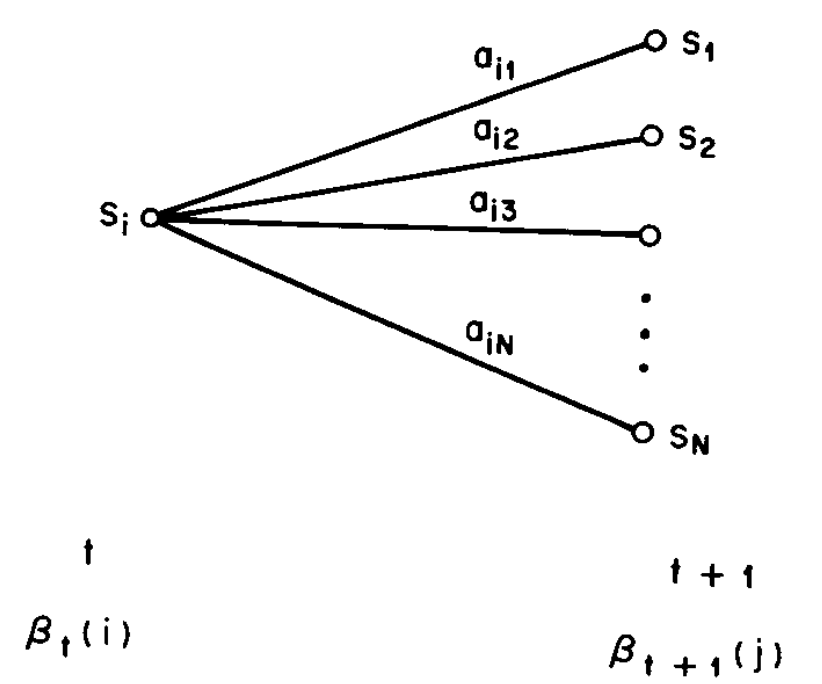
\includegraphics[scale=0.5]{./uploads_new/Hidden_Markov_Model_1._Mo_hinh_Markov_Vi.docx_DIR/media/Fig5.PNG}
\end{center}
\end{figure}


Cũng giống như các biến forward, việc tính tất cả các biến backward cần thực hiện $N^2T$ phép tính. Như vậy, thủ tục forward-backward là khả thi với chi phí tính toán hoàn toàn có thể chấp nhận được.  \par
Đối với việc giải quyết bài toán 1, ta chỉ cần đến phần forward trong thủ tục forward-backward. Về phần backward, ta sẽ gặp lại trong việc giải quyết bài toán 2 và 3. \par

\subsection{\textbf{{Bài toán 2}}}


Mục tiêu của bài toán 2 là tìm ra chuỗi trạng thái   tối ưu Q =  $q_1$, $q_2$, …, $q_T$  đã phát sinh ra O. Một điều đáng lưu ý là có rất nhiều các tiêu chuẩn  tối ưu khác nhau cho việc xác định Q, nên lời giải cho bài toán này phụ thuộc vào tiêu chuẩn tối ưu được chọn.  \par

Trong bài này, ta sử dụng tiêu chuẩn Viterbi. Ta định nghĩa biến $\delta _t(i)$ như sau: 
$$ \delta _t(i) = \max_{q_{1},q_{2},...,q_{t-1}} P \left( q_{1} q_{2} ... q_{t}=i, O_{1} O_{2} ... O_{t} \vert \lambda \right) $$
 là xác suất cao nhất của đoạn chuỗi trạng thái dẫn đến $S_i$ ở thời điểm t và đã quan sát được đoạn $O_1$, $O_2$, …, $O_T$ cho trước mô hình $  \lambda  $

Theo quy nạp, ta có: $$ \delta_{t+1} (j) = \left[\max_i \delta_t(i) a_{ij} \right].b_j \left(O_{t+1} \right) $$

\textbf{Thuật toán Viterbi:} Ta dùng thêm mảng $\psi_t (j)$ để lưu lại tham số i làm cực đại biểu thức.
\begin{enumerate}
\item Khởi tạo:

$$  \delta _{t} \left( i \right) =~ \pi _{i}b_{i} \left( O_{1} \right) ,~1 \leq i \leq N $$

$$  \psi _{1} \left( j \right) =~0 $$

\item Đệ quy: 
\begin{equation}
\delta _{t} \left( j \right) =\max_{1 \leq i \leq N} \left[  \delta _{t-1} \left( i \right) a_{ij} \right] b_{j} \left( O_{t} \right) ,~2 \leq t \leq T,~1 \leq j \leq N
\end{equation}
\begin{equation}
\psi _{t} \left( j \right) =\argmax_{1 \leq i \leq N} \left[  \delta _{t-1} \left( i \right) a_{ij} \right], \quad 2 \leq t \leq T,~1 \leq j \leq N 
\end{equation}

\item Dừng đệ quy: 
$$ P^{*}=\max_{1 \leq i \leq N} \left[\delta_T (i) \right] $$
\[ q_T^{*} = \argmax_{1\leq i \leq N} \left[\delta_T	(i) \right] \]

\item Quay lui: 
$$ q_{t}^{*}= \psi _{t+1} \left( q_{t+1}^{*} \right) ,\quad t=T-1,~T-2,…,~1 $$
\end{enumerate}
Kết thúc thuật toán, chuỗi $ Q=q_{1}^{*}q_{2}^{*}...q_{T}^{*} $
 chính là lời giải của bài toán 2. \par

\subsection{\textbf{{Bài toán 3}}}
Với một chuỗi quan sát hữu hạn bất kỳ O làm dữ liệu luyện, chưa có một phương pháp tối ưu nào cho việc ước lượng các tham số $  \lambda = \left( A,B, \pi  \right)  $ của mô hình theo hướng cực đại toàn cục. Tuy nhiên, bộ tham số $  \lambda  $
 có thể được chọn sao cho xác suất $ p \left( O \vert  \lambda  \right)  $  đạt cực đại địa phương bằng phương pháp Baum-Welch.\par
Trước tiên, ta định nghĩa $  \xi _{t} \left( i,j \right)  $ như sau: 
$$ \xi _{t} \left( i,j \right) =P \left( q_{t}=~S_{i},~q_{t+1}=~S_{j} \vert O, \lambda ~ \right) $$
 là xác suất ở trạng thái $S_i$ tại thời điểm t và rơi vào trạng thái $S_j$ ở thời điểm t+1 cho trước mô hình $  \lambda $ và chuỗi quan sát O. \par
Định nghĩa trên được minh họa bởi hình vẽ sau:
\begin{center}
\begin{figure}[H]
\begin{center}
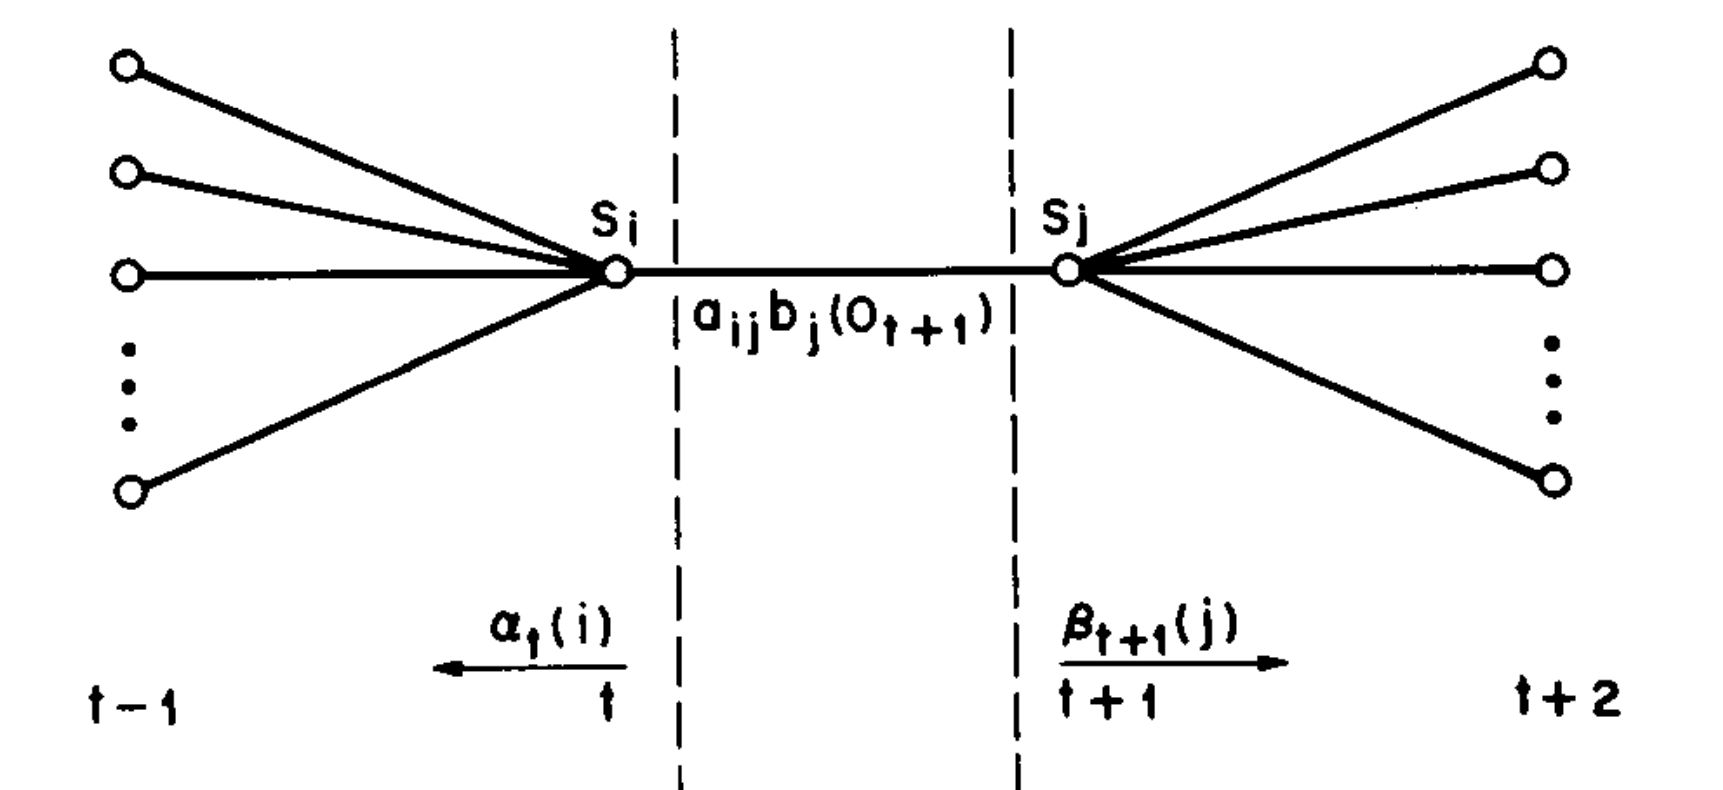
\includegraphics[scale=0.3]{./uploads_new/Hidden_Markov_Model_1._Mo_hinh_Markov_Vi.docx_DIR/media/fig6.PNG}
\end{center}
\end{figure}
\end{center}

Theo định nghĩa này, $ ~ \xi _{t} \left( i,j \right)  $
 có thể được tính thông qua các biến $  \alpha _{t} \left( i \right)  $
 và $  \beta _{t} \left( i \right)  $
 theo công thức:   
 $$\begin{array}{l}
{\xi _t}\left( {i,j} \right) = \frac{{{\alpha _t}\left( i \right){a_{ij}}{b_j}({O_{t + 1}}){\beta _{t + 1}}\left( j \right)}}{{P(O|\lambda )}}
 = \frac{{{\alpha _t}\left( i \right){a_{ij}}{b_j}({O_{t + 1}}){\beta _{t + 1}}\left( j \right)}}{{\mathop \sum \limits_{i = 1}^N \mathop \sum \limits_{j = 1}^N {\alpha _t}(i){a_{ij}}{b_j}({O_{t + 1}}){\beta _{t + 1}}\left( j \right)}}
\end{array}$$ \par

Ta định nghĩa  $\gamma_t(i)$ như sau:
$${\gamma _t}\left( i \right) = p{\rm{(}}{q_t} = {S_{i}}{\rm{|}}O,\lambda )$$

là xác suất ở trạng thái $S_i$ vào thời điểm t cho trước chuỗi tín hiệu quan sát O và mô hình $  \lambda  $. \par
Khi đó, Biến $  \gamma _{t} \left( i \right)  $
 có thể được tính thông qua các biến $  \alpha _{t} \left( i \right)  $
 và $  \beta _{t} \left( i \right)  $
 theo biểu thức: 

$$  \gamma _{t} \left( i \right) =~\frac{ \alpha _{t} \left( i \right) ~ \beta _{t} \left( i \right) }{P \left( O \vert  \lambda  \right) }=\frac{ \alpha _{t} \left( i \right) ~ \beta _{t} \left( i \right) }{\mathop \sum \limits_{i=1}^{N} \alpha _{t} \left( i \right) ~ \beta _{t} \left( i \right) } $$ \par

Vì vậy, ta có thể thấy liên hệ giữa $\gamma_t(i)$ và $ \xi _t(i,j)$: 
$$ \gamma_t(i)=\sum_{j=1}^N \xi_t(i,j) $$ \par
Nếu ta lấy tổng $  \gamma _{t} \left( i \right)  $
 theo $ t~ \in  \left[ 1,T-1 \right]  $
, kết quả nhận được là kỳ vọng của số lần chuyển trạng thái từ $S_i$. Tương tự, lấy tổng $  \xi _{t} \left( i,j \right)  $
 theo $ t~ \in  \left[ 1,T-1 \right]  $
, ta sẽ có kỳ vọng của số lần chuyển từ trạng thái $S_i$ sang $S_j$: \par
\begin{center}

$\mathop \sum \limits_{t = 1}^{T - 1} {\rm{}}{\gamma _t}(i) = $ kỳ vọng của số lần chuyển trạng thái từ $S_{i}$ 
 \par
$\mathop \sum \limits _{t=1}^{T-1}~ \xi _{t} \left( i,j \right) =$ kỳ vọng của số lần chuyển trạng thái từ $S_{i}$ sang $S_{j}~ $
 \par
 
\end{center}
Với các đại lượng này, ta có các biểu thức cập nhật tham số của HMM như sau:
\begin{equation}
{\bar \pi _i}  = \gamma _{1} \left( i \right)  
\end{equation}

\begin{equation}
{\bar a_{ij}} =\frac{ \mathop \sum \limits _{t=1}^{T-1} \xi _{t} \left( i,j \right) }{ \mathop \sum \limits _{t=1}^{T-1} \gamma _{t} \left( i \right) }
\end{equation}

\begin{equation}
{\bar b_j}\left( k \right) = \frac{{\mathop \sum \limits_{t = 1,{O_t} = {v_k}}^T {\gamma _t}(j)}}{{\mathop \sum \limits_{t = 1}^T {\rm{}}{\gamma _t}(j)}}
\end{equation}

Với mô hình ban đầu $  \lambda = \left( A,B, \pi  \right)  $ và chuỗi quan sát O, ta tính được ${\bar{\pi_i}}$, ${\bar{a_{ij}}}$, ${\bar{b_j}}(k)$, kết quả nhận được chính là các tham số mới của mô hình $  \bar{\lambda} = \left( \bar{A},\bar{B}, \bar{\pi}  \right)  $. Theo Baum đã chứng minh, ta luôn có $ p \left( O \vert  \bar{\lambda}  \right) >~p \left( O \vert  \lambda  \right)  $, nếu mô hình $  \lambda  $ đã đạt đến điểm tối ưu địa phương (khi đó $ ~ \lambda =~ \lambda  $). \par
Dựa vào thủ tục trên, nếu ta áp dụng $\bar{\lambda}$ để thay thế $\lambda$ qua nhiều bước lặp thì ta có thể cải thiện xác suất xảy ra O cho đến khi hội tụ. Tuy nhiên, kết quả cuối cùng chỉ đạt được tối ưu địa phương.
\chapter{Mô Hình Gaussian Hỗn Hợp Kết Hợp Markov Ẩn}
Trong chương 1, chúng ta mới chỉ bàn luận đến mô hình Markov ẩn với các quan sát là biến rời rạc. Tuy nhiên đối bài toán đòi hỏi xử lý các tín hiệu âm thanh liên tục, chúng ta cần cải tiến mô hình Markov cho trường này. Vì vậy, chương này sẽ trình bày mô hình Gaussian Hỗn Hợp kết hợp với Markov ẩn

\section{Mô Hình Gaussian Hỗn Hợp}
Mô hình Gaussian hỗn hợp thường được sử dụng để sấp xỉ một hàm mật độ của một biến ngẫu nhiên liên tục nào đó. Mô hình GMM được viết dưới dạng chồng chất của các phân phối chuẩn như sau:
$$p(x) = \sum_{k=1}^{K} \pi_k \mathcal{N}(x | \mu_k, \Sigma_k)$$
trong đó $x$ là một biến ngẫu nhiễn $N$ chiều $\mathcal{N}(x | \mu_k, \Sigma_k)$ là hàm mật độ của biến ngẫu nhiên phân phối chuẩn có kì vọng là $\mu_k$ và ma trận hiệp phương sai $\Sigma_k$. \\

Để thuận tiện cho việc trình bày, ta gọi $z$ là biến ngẫu nhiên nhị phân $K$ chiều, tức là chỉ có một thành phần của $z$ bằng 1 và các thành phần còn lại bằng 0. Như thế, chúng ta thấy rằng chỉ có thể có $K$ khả năng cho biến ngẫu nhiên $z$. Và biến ngẫu nhiên $z$ thỏa mãn tính chất sau:
$$ p(z_k = 1) = \pi_k \ sao \ cho \sum_{k=1}^{K} \pi_k =  1$$
$$p(x|z_k = 1) = \mathcal{N}(x| \mu_k, \Sigma_k)$$
Lý do tạo ra một biến phụ $z$ như vậy là để ta có thể dễ dàng thấy được mỗi liên hệ giữa biến $z$ và các vector quan sát trên một graphical model, và sau này ta thấy rằng việc kết hợp với mô hình markov ẩn chính là việc mở rộng mô hình Gaussian hỗn hợp theo thời gian và các biến $z_i$ tương ứng với các trạng thái. Từ định nghĩa trên, ta có thể viết $p(x)$ dưới dạng sau
$$p(x) = \sum_{z} p(z) p(x | z) = \sum_{k=1}^{K} \pi_k \mathcal{N}(x | \mu_k, \Sigma_k) $$
Một đại lượng khác cũng rất quan trọng là xác suất có điều kiện của biến $z$ khi biết quan sát $x$. Ta kí hiệu
$$\gamma(z_k) = p(z_k = 1| x) = \frac{\pi_k \mathcal{N}(x|\mu_k, \Sigma_k)}{\sum_{j=1}^{K} \pi_k \mathcal{N}(x|\mu_j, \Sigma_j)}$$

Chú ý rằng định nghĩa của biến $\gamma(z)$ rất giống với định nghĩa của biến $\gamma_t(i)$ dùng để chỉ sác xuất của mô hình ở một thái trạng thái nào đó khi biết quan sát đã được miêu tả trong chương 1. \\
Chúng ta có thể hiểu rằng $\pi_k$ là xác suất tiên nghiệm của $z_k = 1$ và $\gamma(z_k)$ là xác suất hậu nghiệm khi mà ta đã nhìn thấy được một quan sát $x$.
\subsection{Hợp Lí Cực Đại}
Giả sử có một dãy quan sát $\{ x_1, x_2, ..., x_N\}$, ta có thể biểu diễn dữ liệu này bằng một ma trận $X$ cỡ $N \ * \ D$. Nếu ta có thêm giả thiết rằng các quan sát này được lấy từ các biến ngẫu nhiên độc lập có cùng phân phối, khi đó ta có thể biểu diễn phân phối đó theo một mô hình Gaussian hỗn hợp với hàm loga hợp lý như sau
$$ln \ p(X| \pi, \mu, \Sigma) = \sum_{n=1}^{N} ln \Bigg\{\sum_{k=1}^{K}\pi_k \mathcal{N}(x_n| \mu_k, \Sigma_k)\Bigg\}$$

Bài toán đặt ra là tìm các tham số $\pi, \mu$ và ma trận hiệp phương sai $\Sigma$ làm cực đại hàm loga trên. Và một trong những phương pháp có ứng dụng rộng rãi để giải quyết bài toán trên là phương pháp cực đại kì vọng (Expectation Maximization - EM)
\subsection{Cực Đại Kì Vọng}
Đạo hàm hàm loga hợp lý $ln \ p(X| \pi, \mu, \Sigma)$ theo biến $\mu_k$ ta có
$$\sum_{n=1}^{N} \frac{\pi_k \mathcal{N}(x_n| \mu_k, \Sigma_k)}{\sum_j \pi_j \mathcal{N}(x_n | \mu_j, \Sigma_j)} \ \Sigma_{k}^{-1}(x_n - \mu_k) = 0 $$
\begin{center}
hay
\end{center}
$$\sum_{n=1}^{N} \gamma(z_{nk}) \ \Sigma_{k}^{-1}(x_n - \mu_k)$$
Nhân hai vế với $\Sigma_k$, ta có :
$$\mu_k = \frac{1}{N_k} \sum_{n=1}^{N} \gamma(z_{nk)} \ x_n$$
trong đó $N_k$ được định nghĩa như sau :
$$N_k = \sum_{n=1}^{N} \gamma(z_{nk})$$
Chúng ta có thể hiểu $N_k$ như là số các điểm được phân loại vào phân cụm $k$. Chú ý rằng từ công thức trên, kì vọng $\mu_k$ của thành phần Gaussian thứ $k$ được tính bằng trung bình có trọng số của những điểm trong dữ liệu, với trọng số được tính phụ thuộc vào xác suất hậu nghiệm $\gamma(z_{nk})$. \\
Tương tự, vì đạo hàm $ln \ p(X| \pi, \mu, \Sigma)$ theo $\Sigma_k$ bằng không, ta thu được
$$\Sigma_k = \frac{1}{N_k} \sum_{n=1}^{N} \gamma(z_{nk})(x_n - \mu_k)(x_n - \mu_k)^T$$
Cuối cùng, để tối ưu hàm $ln \ p(X| \pi, \mu, \Sigma)$ theo hệ số $\pi_k$, ta phải để ý đến rằng buộc $\sum_k \pi_k = 1$. Để giải quyết vấn đề này ta tối ưu hàm Langrange sau
$$ln \ p(X| \pi, \mu, \Sigma) + \lambda (\sum_{k=1}^{K} \pi_k - 1)$$
Đạo hàm theo $\pi_k$ ta được
$$\sum_{n=1}^{N} \frac{\pi_k \mathcal{N}(x_n| \mu_k, \Sigma_k)}{\sum_j \pi_j \mathcal{N}(x_n | \mu_j, \Sigma_j)} + \lambda = 0$$
Nhân hai vế với $\pi_k$ và lấy tổng theo $k$, ta được
$$\pi_k = \frac{N_k}{N}$$
Tuy rằng những kết quả này không thể thiết lập được công thức cho việc tối ưu hàm loga hợp lý, nhưng những công thức trên lại có thể được sử dụng trong các vòng lặp để các tham số có thể tiến đến nghiệm tối ưu địa phương của bài toán.\\
Đầu tiên, ta chọn ra các giá trị khởi đầu cho $\pi, \mu$ và $\Sigma$ và ta thực hiện các vòng lặp gồm 2 bước E (Expectation) và M (Maximization). Ở trong bước E, ta sử dụng các giá hiện tại để tính xác suất hậu nghiệm $\gamma_(z)$, sau đó sử dụng các công thức trên để tính lại các giá trị $\pi, \mu$ và $\Sigma$. Và người ta đã chứng minh được rằng với cách làm như vậy thì hàm loga hợp lí sẽ tăng sau mỗi bước lặp. Nhận xét rằng việc thay đổi các giá trị kì vọng của các phân phối chuẩn tương đương với việc tìm ra các tâm của các phân cụm có trong dữ liệu. Vì vậy ta thấy rằng nếu biểu diễn một hàm mật độ thông qua mô hình này, sẽ tốt hơn so với việc phân cụm các vector và chuyển các quan sát từ dữ liệu liên tục thành rời rạc. Lí do ở chỗ khi phân cụm như vậy thì ta đã bị mất đi thông tin rằng dữ liệu thử của chúng ta cách xa tâm bao nhiêu và vì vậy dễ dẫn đến nhầm lẫn
\section{Mô Hình Gaussian Hỗn Hợp Kết Hợp Markov Ẩn}
Chương 1 đã miêu tả thuật toán Baum-Welch để tối ưu các tham số của mô hình Markov ẩn đối với 1 dãy quan sát và các tín hiệu ở đây là rời rạc. Tuy nhiên, khi giải quyết bài toán xử lý âm thanh, ta phải đối mặt với hai vấn đề, thứ nhất là các tín hiệu âm thanh là liên tục và thứ hai là ta nếu có nhiều dãy dữ liệu luyện thì sao. Mục này sẽ trình bày cách giải quyết hai vấn đề trên. \\
Trong phần trước, ta đã thấy rằng mô hình Gaussian hỗn hợp được sử dụng để xấp xỉ một hàm mật độ nào đó, và khi có một dãy các quan sát ta đã có thuật toán EM để cực đại hàm hợp lí. Và một cách tự nhiên, ta sẽ sử dụng mô hình này để xấp xỉ hàm mật độ xác suất đầu ra của mỗi trạng thái trong mô hình Markov ẩn, có nghĩa là $b_j(O)$ của chúng ta bây giờ có dạng
$$b_j(O) = \sum_{m=1}^M c_{jm} \mathcal{N}(O| \mu_{jm}, \Sigma_{jm})$$
trong đó $O$ là một quan sát, $M$ là số thành phần Gaussian, $N$ là số trạng thái trong mô hình Markov ẩn, và $c_{jm}$ là hệ số của các thành phần $Gaussian$ ứng với trạng thái $j$. Và tất nhiên các hệ số phải thỏa mãn ràng buộc
$$\sum_{m=1}^{M} c_{jm} = 1 \ \ \ \forall 1 \leq j \leq N$$
$$c_{jm} \geq 0 \ \ \ \ \ \forall 1 \leq N, 1 \leq m \leq M$$
Khi đó các công thức để tính lại tham số của mô hình Gaussian hỗn hợp trở thành

\begin{equation}
    \overline{c_{jk}} = \dfrac{\sum\limits_{t=1}^{T} \gamma_{t}(j, k)}{\sum\limits_{t=1}^{T} \sum\limits_{k=1}^M \gamma_t(j, k)}
\end{equation}

\begin{equation}
\overline{\mu_{jk}} = \dfrac{\sum\limits_{t=1}^{T} \gamma_t(j, k) O_t}{\sum\limits_{t=1}^{T} \gamma_t(j,k)}
\end{equation}

\begin{equation}
\overline{\Sigma_{jk}} = \frac{\sum\limits_{t=1}^{T} \gamma_t(j, k) \ (O_t - \mu_{jk}) (O_t - \mu_jk)^T}{\sum\limits_{t=1}^T \gamma_t(j, k}
\end{equation}

Bây giờ, ta chi còn phải xem xét đối với trường hợp có nhiều dữ liệu luyện thì quá trình cập nhập tham số của thuật toán Baum-Welch sẽ như thế nào. Kí hiệu
$$ O = [O^{(1)}, O^{2}, \dots, O^{k}]$$
trong đó $O^{k} = [O_1^{k}, O_2^{k}, \dots, O_{t_k}^{k}]$ là dãy quan sát thứ $k$ gồm $t_k$ quan sát. Với giả thiết rằng các dãy quan sát này là độc lập, và mục đích của chúng ta là tìm các tham số của mô hình Markov ẩn làm cực đại

$$P(O | \lambda) = \prod_{k=1}^K P(O^{k} | \lambda) = \prod_{k=1}^K P_k$$

Từ đó, ta có các công thức ước lượng ma trận xác suất chuyển $A$ và xác suất đầu ra tại mỗi trạng thái như sau

\begin{equation}
\overline{a_{mn}} = \dfrac{\sum\limits_{k=1}^k \sum\limits_{t=1}^{t_k} \xi_t(m,n)}{\sum\limits_{k=1}^K \sum\limits_{t=1}^{t_k} \gamma_{t}^{k}(m)}
\end{equation}

\begin{equation}
\overline{b_n(m)} = \dfrac{\sum\limits_{k=1}^K \sum\limits_{t = 1, o_t^{k} = v_m}^{t_k} \gamma_{t}^{k}(n)}{\sum\limits_{k=1}^K \sum\limits_{t = 1}^{t_k} \gamma_{t}^{k}(n)}
\end{equation}

\begin{equation}
\overline{\pi_n} = \dfrac{1}{K} \sum_{k=1}^{K} \gamma_1^{k}(n)
\end{equation}

Các đại lượng $\overline{c_{jk}}, \overline{\mu_{jk}}, \overline{\Sigma_{jk}}, \overline{a_{mn}}, \overline{b_n(m)}$ và $\overline{\pi_n}$ được thực hiện tính lặp đi lặp lại theo các công thức từ (2.1) đến (2.6) đến khi thì được nghiệm tối ưu địa phương của bài toán cực đại hàm $P(O | \lambda)$. 
\chapter{Âm Thanh - Thuật Toán MFCC}
Tín hiệu âm thanh ngoài đời thực là một chuỗi âm liên tục. Âm thanh được lan truyền trong vật chất giống như các sóng. Âm thanh, giống như nhiều sóng, có 2 đặc trưng chính là biên độ và tần số. \\
Trước khi thực hiện bất cứ bước xử lý nào, tín hiệu âm thanh cần được số hóa do máy không thể lưu lại âm thanh thực. Việc này được thực hiện tự động bởi các thiết bị thu âm, bằng cách lấy mẫu tín hiệu đầu vào (như máy ghi âm, điện thoại, máy tính,v.v). Lưu trữ tín hiệu âm thanh trên thiết bị thu âm yêu cầu tách tín hiệu thành một khoảng thời gian và tính toán giá trị biên độ trung bình cho mỗi khoảng thời gian đó. 

\begin{figure}[H]
\begin{center}
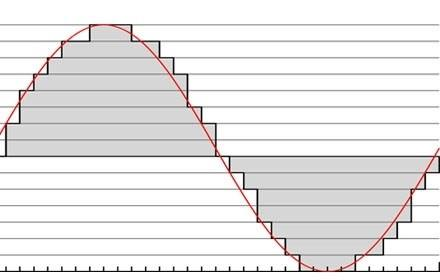
\includegraphics[scale=0.5]{./uploads_new/Hidden_Markov_Model_1._Mo_hinh_Markov_Vi.docx_DIR/media/anh1.jpg}
\end{center}
\end{figure}

Giả sử chúng ta có một tệp / luồng với dữ liệu âm thanh. Trước hết chúng ta cần phải hiểu cấu trúc bên trong của nó và cách nó có thể được đọc. Hãy xem xét trường hợp đơn giản nhất - một tệp WAV.\\
Định dạng này bao hàm sự hiện diện của hai khối trong tệp. Đầu tiên là tiêu đề với thông tin của luồng âm thanh: tốc độ bit, tần số, số lượng kênh, độ dài của tệp, v.v. Dữ liệu thứ hai chứa dữ liệu "thô" - tín hiệu số, bộ giá trị biên độ của tín hiệu.\\
Cách đọc trong trường hợp này khá đơn giản. Đọc tiêu đề, kiểm tra một số hạn chế (ví dụ không nén), lưu trữ dữ liệu vào một mảng đặc biệt.

Đầu tiên, ta chia nhỏ dữ liệu âm thanh thành một tập hợp các khoảng thời gian nhỏ - khung. Lưu ý rằng, khung không nên được chia thành các đoạn riêng lẻ; thay vào đó chúng nên được chia "chồng lên nhau". Hay nói cách khác, kết thúc của khung n phải giao với đầu của khung n+1\\
Một lý do khác cho thấy sự cần thiết của việc chia khung là vì tín hiệu âm thanh thay đổi rất nhanh, do đó các thuộc tính như biên độ, chu kỳ sẽ không ổn định. Khi tín hiệu âm thanh được cắt ra thành những đoạn nhỏ thì ở mỗi đoạn, có thể coi tín hiệu đó là ổn định, các đặc trưng của tín hiệu thay đổi nhỏ theo thời gian.
\section{Phường Pháp MFCC}
Trong nhận dạng tiếng nói, kỹ thuật trích chọn đặc trưng MFCC là phương pháp phổ biến nhất. MFCC là viết tắt của Mel-frequency cepstral coefficients. Kỹ thuật này dựa trên việc thực hiện biến đổi để chuyển dữ liệu âm thanh đầu vào (đã được biến đổi Fourier cho phổ) về thang đo tần số Mel, một thang đo diễn tả tốt hơn sự nhạy cảm của tai người đối với âm thanh. Kỹ thuật trích chọn đặc trưng này gồm các bước biến đổi liên tiếp, trong đó đầu ra của bước biến đổi trước sẽ là đầu vào của bước biến đổi sau. Đầu vào của quá trình trích chọn đặc trưng này sẽ là một đoạn tín hiệu tiếng nói. Vì tín hiệu âm thanh sau khi được đưa vào máy tính đã được rời rạc hóa nên đoạn tín hiệu tiếng nói này bao gồm các mẫu liên tiếp nhau, mỗi mẫu là một giá trị thực, thể hiện giá trị biên độ của âm thanh tại 1 thời điểm.\\

Ta gán khung như một vecto: $x[k],\quad 0 \leq k \leq N$ trong đó $N$ là kích thước của nó.\\
Đầu tiên là thực hiện biến đổi Fourier rời rạc đối với từng phổ của tín hiệu đã được cắt ra. Qua phép biến đổi này, tín hiệu sẽ được đưa về không gian tần số. Công thức của biến đổi Fourier:
$$X[k]=\sum_{n=0}^{N-1}x[n]e^{-2 \frac{\pi}{N} ikn, \quad 0\leq k < N}$$
\\
Cùng với đó, ta sử dụng hàm "cửa sổ" Hamming để làm "mượt" các giá trị ở hai đầu mút của khung:
$$H[k]=0.54-046\cos\left(\frac{2\pi k}{N-1}\right)$$\\
Kết quả là chúng ta có vecto sau:
$$X[k]=X[k]*H[k], \quad 0\leq k <N$$\\

Kết quả của quá trình biến đổi Fourier thể hiện năng lượng của tín hiệu ở những dải tần số khác nhau. Tuy nhiên, tai của người lại không có sự nhạy cảm như nhau đối với mọi dải tần số. Do đó việc mô hình hóa tính chất này của tai người trong quá trình trích chọn đặc trưng làm tăng khả năng nhận dạng của hệ thống. Trong mô hình trích chọn đặc trưng MFCC, tần số sẽ được chuyển sang thang đo tần số mel theo công thức:
$$M=1127*log\left(1+\frac{F}{700}\right)$$
Từ công thức trên, biến đổi ta được:
$$F=700\left(e^{\frac{M}{1127}}-1\right)$$
\\
Vì chúng ta biết số lượng các hệ số và dải tần số, nên ta có thể xây dựng các bộ lọc sau đây:
\begin{figure}[H]
\begin{center}
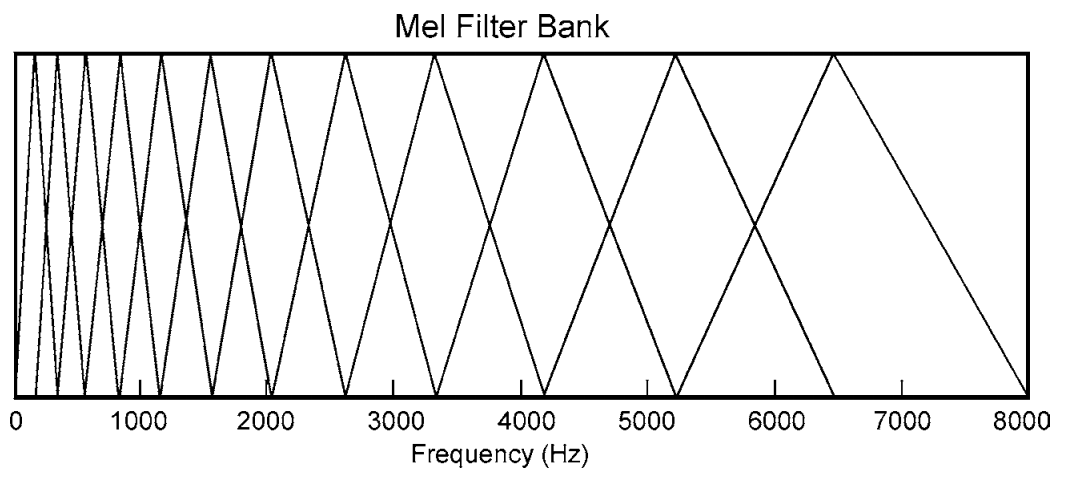
\includegraphics[scale=0.3]{./uploads_new/Hidden_Markov_Model_1._Mo_hinh_Markov_Vi.docx_DIR/media/anh2.png}
\end{center}
\end{figure}

Cuối cùng, ta có thể xây dựng được bộ lọc cần thiết theo công thức sau:
\begin{align}{H_m(k)=}
\nonumber
    \begin{cases}
        0 \quad \quad \quad \quad \quad \quad k<f(m-1) \\
        \frac{k-f(m-1)}{f(m)-f(m-1} \quad f(m-1)\le k \le f(m) \\
        \frac{f(m+1)-k}{f(m+1)-f(m)} \quad f(m)\le k \le f(m+1)\\
        0 \quad \quad \quad \quad \quad \quad k>f(m+1)
    \end{cases}
\end{align}

trong đó: $$f(i)=floor\left(\frac{(frameSize+1)h(i)}{sampleRate}\right)$$
\\
Tổng của các phần tử trong vecto có kết quả là một hệ số mel. Vì chúng ta có M bộ lọc, số lượng các hệ số là như nhau, ta có: 
$$S(m)=\log\left(\sum_{k=0}^{N-1} |X(k)|^2 H_m(k)\right), \quad 0\le m <M$$
Do ta áp dụng bộ lọc mel cho năng lượng chứ không phải cho phổ nên cần lấy logarit kết quả. Và bằng cách  này, ta tin rằng nó có thể làm giảm độ nhiễu của tiếng ồn.
\section{Biến đổi Cosin}
Bước tiếp theo của việc trích chọn đặc trưng MFCC là biến đổi fourier ngược với đầu vào là các hệ số phổ mel của bước trước, đầu ra sẽ là các hệ số cepstrum (MFCC – Mel Frequency Cepstrum Coefficients):
$$C(l)=\sum_{m=0}^{M-1} S(m)\cos\left(\frac{\pi L(m+\frac{1}{2}}{M}\right), \quad 0\le l<M$$

\chapter{Mô Hình Nhận Diện Từ Đơn}
Trong chương này, bài báo cáo trình bày về mô hình sử dụng HMM trong việc nhận dạng từ đơn Tiếng Việt. Giả sử ta cần nhận diện các từ trong một bộ từ điển gồm $V$ từ. Chúng ta luyện một mô hình Markov ẩn riêng cho mỗi từ trong từ điển. Có nghĩa là với mỗi từ, ta có một số lượng $K$ ghi âm của từ đó. Như ở chương trước đã trình bày, với mỗi một tín hiệu âm thanh, ta có thể thu được một chuỗi các vector liên tục tự thuật toán MFCC như trình bày ở trên. Áp dụng thuật toán này lên tất cả các bản ghi âm của từng từ, ta được một bộ gồm $K$ chuỗi vector. Các bộ này sẽ được sử dụng như là các dãy quan sát để luyện cho mô hình Markov ẩn. Noi ngắn gọn, mô hình nhận diện được thực hiện qua hai bước sau:
\begin{enumerate}
\item Với mỗi một từ $v$ ở trong từ điển, ta xậy dưng một mô hình Markov ẩn $(A, B, \pi)$ dựa vào phương pháp tối ưu đã được trình bày ở chương 1 và chương 2. Tức là ở bước này, ta đã có $V$ mô hình với mỗi từ có trong từ điển 
\item Để nhận dạng một từ không có trong bộ dữ liệu luyện, đầu tiên, từ đó được tiền xử lý, sau đó được phân tích thành các vector dựa vào MFCC. Khi đó ta thu được một quan sát $O = [O_1, O_2, \dots, O_T]$. Ta tính xác suất $P(O | \lambda_v)$ với tất cả các mô hình có trong hệ thống, và coi như các xác suất tính được như giá trị đánh giá độ hợp lý của dãy quan sát $O$ được sinh ra bơi mô hình đó. Và hệ thống sẽ chọn $v^* = \argmax_{1 \leq v \leq V} P(O | \lambda_v)$ và kết luận $v^*$ là chữ nhận diện được. \\
\end{enumerate}
Hệ thống được mô tả bằng hình vẽ sau đây \\
\includegraphics[scale=0.55]{./model.PNG} \\

Để luyện các model cho từng từ, việc chọn số hidden state, rằng buộc giữa các state, số lượng khung (frame) và khoảng cách của các khung khi xử lý dữ liệu có ảnh hướng lớn đến kết quả nhận diện của hệ thống. Vì cơ sở lý thuyết của mô hình Markov chưa chỉ rằng được số lương trạng thái ẩn và số gaussian mixture là bao nhiêu thì có thể đạt được model của. Do đó nhưng tham số trên được chọn dựa trên thực nghiệm. Tuy nhiên ta có thể hiểu ngầm rằng, các trạng thái ẩn tương ứng với các chữ cái, còn các quan sát là các cách phát âm của các chữ cái đó.

\chapter{Kết Quả Thực Nghiệm}
Để thử nghiệm mô hình, chung tôi thực hiện trên một bộ dữ liệu mẫu bao gồm ghi âm của các từ là số đếm từ 0 đến 9. Tập dữ liệu gồm 18 file chỗ mỗi số. Khi thực hiện luyện cho một model tương ứng với mỗi số 14 file được lấy ngẫu nhiên làm dữ liệu luyện và 4 file còn lại được lấy làm dữ liệu kiểm thử (test). Các file ghi âm đều được xử lý thông qua phương pháp trích phổ MFCC. Ví dụ một file .wav và các tin hiệu âm thanh sau khi được xử lý để làm dữ liệu luyện và kiểm thử \\
\begin{center}
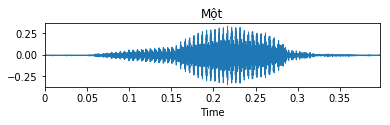
\includegraphics[scale=.9]{wave.png} \\
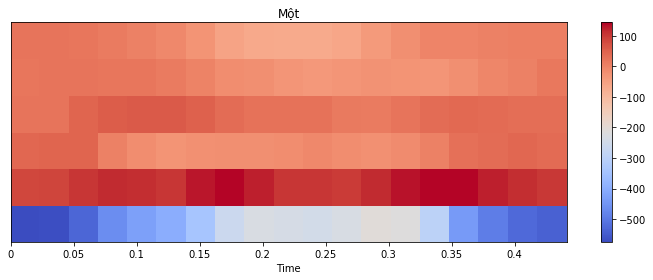
\includegraphics[scale=.6]{mfcc.png}
\end{center}

Như đã trình bày ở chương trước, không có lý thuyết vững vàng cho việc chọn số lượng trạng thái, số lượng các phẩn phối chuẩn, độ dài của khung (frame) và độ dài phần trùng nhau giữa các khung. Vì vậy cách làm ở đây là duyệt qua các tham số và chọn ra bộ tham số có kết quả tốt nhất. \\

Bảng sau lưu lại một số setting của tham số và kết quả của mô hình \\ 
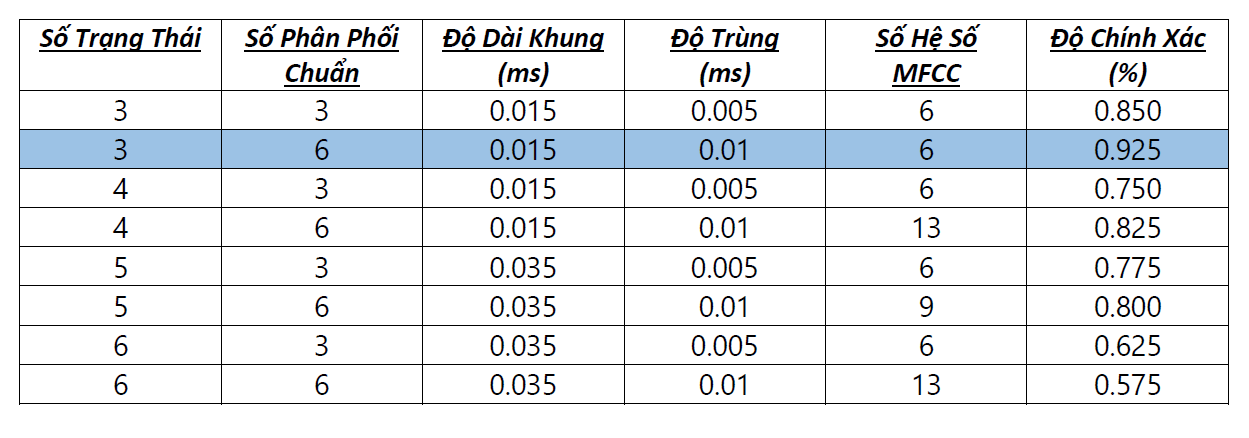
\includegraphics[scale=.6]{thongke.PNG} \\
Ma trận nhầm lẫn của mô hình thứ 2 trong bảng \\
\begin{center}
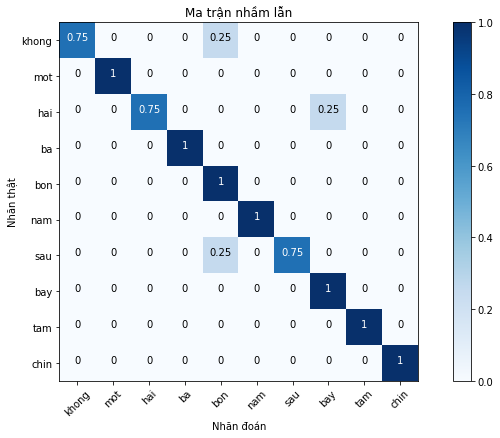
\includegraphics[scale=.5]{confumatrix.png}
\end{center}
Ta có thể thấy model nhận diện các dữ liệu kiểm thử khá tốt. Tuy nhiên khi xem xét kĩ nhứng trường hợp đó, ta thấy rằng những giá trị để hàm $P(O | \lambda)$ tốt thứ hai là đáp án đúng.

Mô hình nhân diện từ đơn của nhóm được tải lên 
\href{url}{https://github.com/hidevn/hmm}





 
\chapter{Kết luận}
Trong báo cáo này, chúng tôi đã gợi thiệu và trình bày khái niệm về mô hình Markov ẩn và cách kết hợp mô hình Gaussian hỗn hợp vào mô hình markov ẩn nhằm biểu diễn sự liên tục của biến quan sát ứng với mỗi trạng thái. Bên cạnh đó, bài báo cáo đã trình bày về cách xử lý tín hiệu âm thanh và xây dừng hệ thống giúp nhận diện từ đơn trong Tiêng Việt. Kết quả thu được khá tốt đối với bộ dữ liệu gồm 10 từ để nhận diện số. \\
Đối với Tiếng Việt, việc nhận diện được từ đơn khá quan trọng khi tất các câu nói đều cấu thành từ các âm riêng lẻ. Một hướng phát triển tiếp khi đã có được một model nhận diện từ đơn tốt là phương pháp tách từ. Công việc tách từ cũng hoàn toàn có thể thực hiện được nhờ mô hình Markov, tuy nhiên do hạn chế về thời gian nên nhóm chúng tối chưa thể giải quyết của bài toán này. \\
Một nhược điểm dễ thấy của mô hình này là khi số lượng từ trong từ điển lớn thì hệ thống sẽ xử đi chậm đi rất nhiều do nhiều lần phải tính $P(O| \lambda)$. Và hướng làm tiếp theo của nhóm là muốn giải quyết vấn đề này, với ý tưởng rằng ta có thể nhận diện chữ cái thay cho việc nhận diên từ đơn vì cách phát âm của Tiếng Việt là hoàn toán có quy tắc. \\
Lời cuối cùng, cho phép chúng tôi cảm ơn những người bạn đã giúp đỡ giúp chúng tôi có thể hoàn thành bài báo cáo đúng hạn :)

\newpage
%Tài liệu tham khảo
\begin{thebibliography}{12}
\addcontentsline{toc}{chapter}{\quad\  \bf Tài liệu tham khảo}
\bibitem{1}A Tutorial on Hidden Markov Models and Selected Applications in Speech Recognition\\
\textit{LAWRENCE R. RABINER, IEEE}
\bibitem{2} $http://practicalcryptography.com/miscellaneous/machine-learning/guide-mel-frequency-cepstral-coefficients-mfccs/$.
\bibitem{3}Pattern Recognition and Machine Learning \\
\textit{CHRISTOPHER M. BISHOP}
\bibitem{4}Training Hidden Markov Models with Multiple
Observations - A Combinatorial Method \\
\textit{Xiaolin Li, Member, IEEE}
\bibitem{5}$http://trustmeiamadeveloper.com/2014/06/24/speach_recognition/$




\end{thebibliography}


\end{document}
